% Template for ICIP-2014 paper; to be used with:
%          spconf.sty  - ICASSP/ICIP LaTeX style file, and
%          IEEEbib.bst - IEEE bibliography style file.
% --------------------------------------------------------------------------
\documentclass{article}
\usepackage{spconf,amsmath,graphicx,wrapfig}
\usepackage{hyperref}
\usepackage{caption}
\usepackage{subcaption}

% Example definitions.
% --------------------
\def\x{{\mathbf x}}
\def\L{{\cal L}}

% Title.
% ------
\title{SVETLANA: a Supervised Segmentation Classifier for Napari}
%
% - STALIN
% - SALSIFI
% - SALSA
% - SCAN
% 
% ---------------
\name{Clément Cazorla, Pierre Weiss, Renaud Morin\thanks{Thanks to XYZ agency for funding.}}
\address{Imactiv-3D, IMT}
%
% Two addresses (uncomment and modify for two-address case).
% ----------------------------------------------------------
\twoauthors
 {Clément Cazorla, Renaud Morin \sthanks{C. Cazorla is partially funded by ANR CIFRE 2020/0843. He acknowledges the image.sc community for their precious help.}}
	{IMACTIV-3D\\
	1 place Pierre Potier, 31100 - Toulouse}
 {Pierre Weiss \sthanks{P. Weiss acknowledges a support from ANR-3IA Artificial
and Natural Intelligence Toulouse Institute and ANR Micro-Blind}}
	{CNRS \& Université de Toulouse\\
	31400 - Toulouse}

\begin{document}
%\ninept
%
\maketitle
%
\begin{abstract}
We develop and present a Napari plugin called SVETLANA (SuperVised sEgmenTation cLAssifier for NapAri). It is dedicated to the manual or automatic classification of segmentation results, with a primary focus on bio-medical imaging.
While many open-source softwares now make it possible to automatically segment complex 2D and 3D objects such as cells in biology, the subsequent analysis of the results is not yet accessible to non specialists. 
This plugin allows end-users to train and run efficient neural network classifiers such as residual networks. 
The resulting network can be used as a post-processing tool to improve the segmentation, or as a classifier for various tasks (e.g. separating different cells populations).
We showcase its practicality through various real cell biology problems in 2D, 3D and multi-spectral imaging.
\end{abstract}
%
\begin{keywords}
Software, Segmentation, Classification, Convolutional Neural Networks, Bio-medical imaging, Image analysis
\end{keywords}
%
\section{Introduction}
\label{sec:intro}

The last decade has made automatic segmentation of bio-medical images much more accessible to users not familiar with signal processing. 
This is the result of progress in machine learning, to the creation of open training databases and to the development of ergonomic open-source softwares. Technologies such as neural networks provide unprecedented segmentation results. They make it possible to avoid setting hyperparameters which are often hard to tune and interpret. 
Examples of powerful and popular tools for segmentation in biology include Ilastik \cite{berg2019ilastik}, CellPose \cite{stringer2021cellpose}, StarDist \cite{fazeli2020automated} or Deep-ImageJ \cite{gomez2021deepimagej}. 

\subsection{Our motivation}

Unfortunately, segmentation masks -- as good as they are -- are rarely directly exploitable to answer biological questions. In particular, it is often necessary to classify the detected objects in order to perform statistical analyses that give a concrete meaning to the results. 
While these excellent segmentation tools have solved an important problem, a difficult part of the analysis remains inaccessible to most users.

\subsection{Our contribution}

The goal of this work is to continue filling the gap between methodological advances and end-users, by providing a convenient software for the classification of segmentation results. 
We resort to the newborn Napari environment \cite{perkel2021python} which allows visualizing and analyzing complex multi-dimensional images (e.g. 2D, 3D, 3D+t, hyperspectral) in Python.
Our software takes the form of a Napari plugin called SVETLANA. A screenshot of the plugin is displayed in Fig. \ref{fig:interface}.

\begin{figure}[htp!]
 \centering
 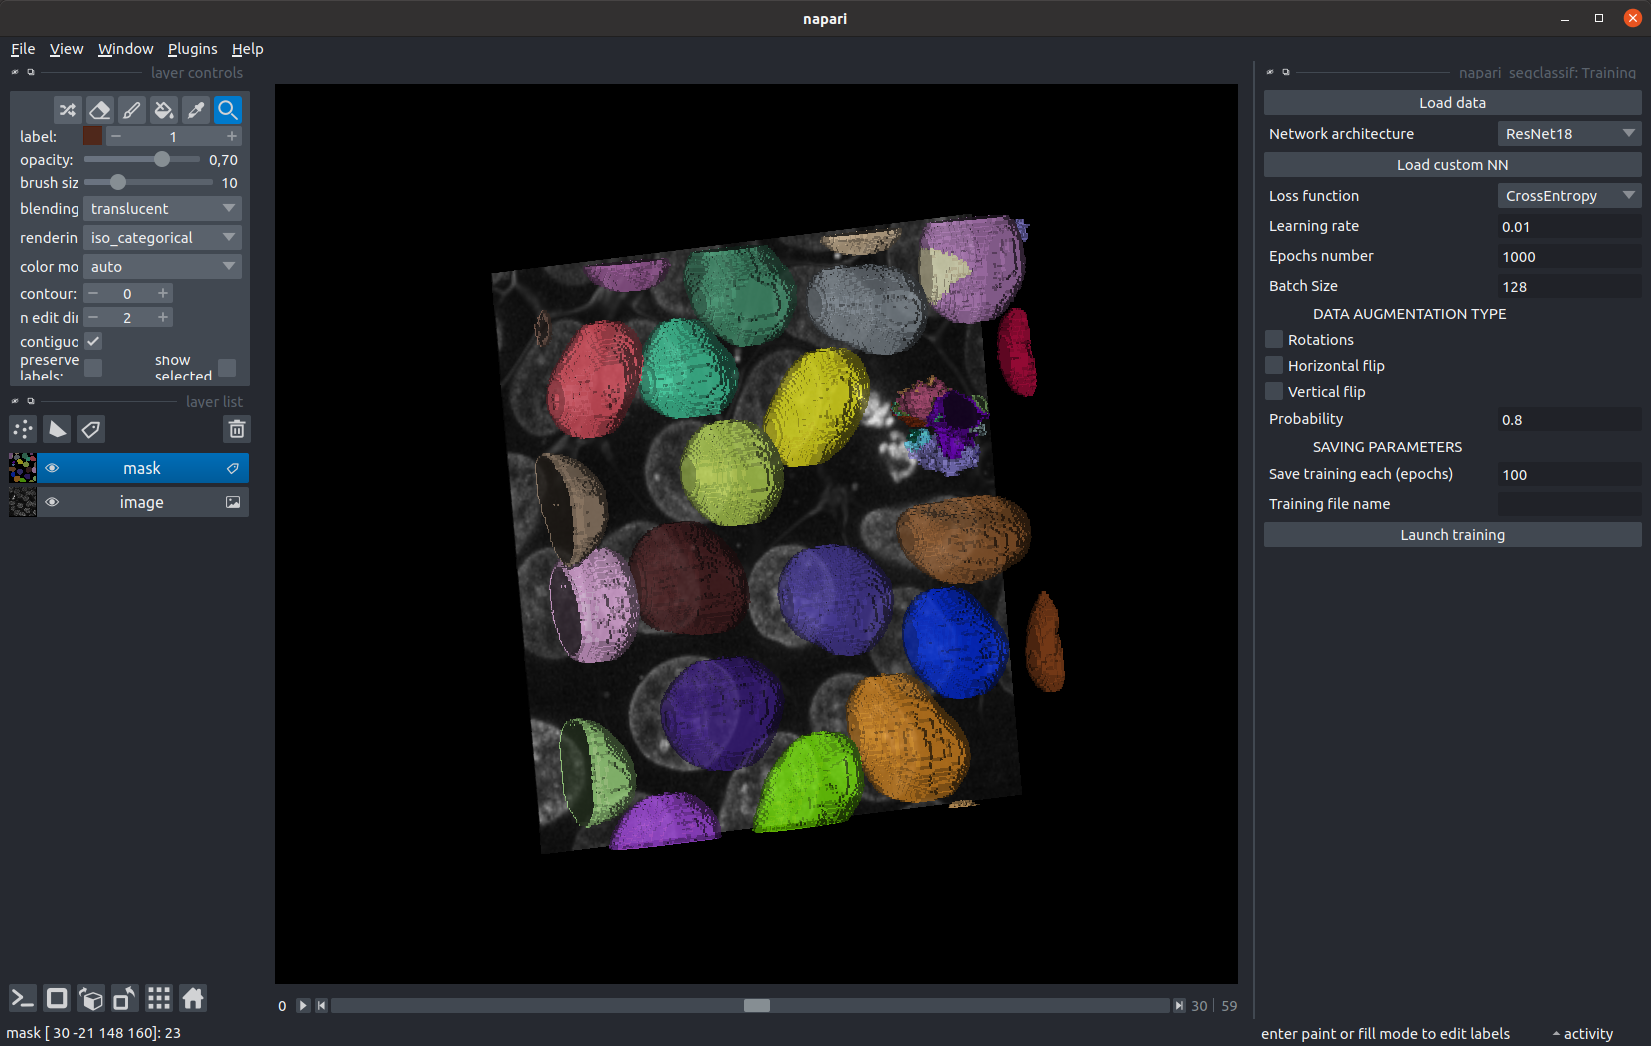
\includegraphics[width=\linewidth]{Figures/interface.png}
  \caption{The SVETLANA plugin under NAPARI. \label{fig:interface}}
  \label{labelization}
\end{figure}

For the input, it takes \emph{an image to label and a segmentation mask}. It is then separated in three different modules: 
\begin{description}
  \item[\emph{Annotation}] This module allows to label connected components of the segmentation masks. In our 2D experiments, it allows labeling about 1000 connected component in 15 minutes.
  \item[\emph{Training}] This module allows to pick an arbitrary Pytorch \cite{paszke2019pytorch} neural network architecture (possibly pretrained) and to further train it with the annotations generated by the previous module.
  \item[\emph{Prediction}] This module uses the trained network to classify the connected components of the segmentation mask.
\end{description}
The outputs of the plugin are: \emph{a set of manually annotated patches, a trained neural network and a prediction mask}. 
The results are stored in files widely accessible formats for the forth-coming analyzes. This plugin meets a need to further enhance the excellent results obtained with recent, wide purpose segmentation tools.

\subsection{Related works}

Different options can be adopted to segment and classify objects in images. 
Before 2010, most of the works relied on the following pipeline (see e.g. \cite{irshad2013methods}): 1) Segment the image 2) Annotate the resulting masks 3) Extract features within the masks (e.g. edges, textures, ...) 4) Design a classifier based on the extracted features. 
Each of the above step was carried out with carefully hand-crafted methods. 
Supervised and unsupervised learning then progressively entered in the game. 
In many cases, they outperformed man-made routines by allowing to explore a wider range of decision routes. 

An effort was then pursued to make these technologies available to the larger number. One remarkable example is Ilastik \cite{berg2019ilastik}. There, a few annotations by the user are usually enough to perform complex classification tasks with an arbitrary number of classes. Its backbone is a random forest classifier with a fixed number of features (convolutions with different filter types). It is widely praised for its ease of use. A few clicks are enough to solve many real-world problems. Unfortunately, this strength is also a limitation in certain cases: the performance of random forests falls short in comparison with the most advanced segmentation and classification routines trained with vast collection of carefully labelled data. 

When precision is critical, the rapidly evolving state-of-the-art is rather based on neural networks and especially convolutional neural networks \cite{dhillon2020convolutional,8237584}. The downside of these technologies is the need to create large data sets, which are usually just not accessible. Each biology laboratory explores a different organism, at a different scale with a different modality and focus. Each collected image can be costly both in terms of money, know-how and time. To address this issue, new initiatives emerge to collect large heterogeneous training databases. For instance the Data Science Bowl \cite{caicedo2019nucleus} allowed to train a single neural network, which is now capable of segmenting cells of nearly any type. This tool, embedded in neat graphical interfaces (e.g. CellPose \cite{stringer2021cellpose} or StarDist \cite{fazeli2020automated}) is a huge asset for biology. Unfortunately, as of now, it does not provide classification tools.

The proposed ideas can be seen as a two-step procedure to classify complex objects. First, we use a general purpose segmentation routine trained with a huge dataset. This highly simplifies the classification task by having to focus only on the right objects. Then train a classifier with just a few annotations (e.g. 100-1000) to sort the resulting objects. As far as we are aware of, this principle is not yet made available as an open-source software.

\section{Plugin description}
\label{sec:format}

The objective of SVETLANA as a whole is to provide a tool targeted to people not familiar with programming to "sort" the segmentation results, either manually or automatically. 

\subsection{The choice of Napari}
The specifications were:
\begin{itemize}
  \setlength{\itemsep}{3pt}%
  \setlength{\parskip}{0pt}%
  \item Use highly parallel architectures for run-time efficiency.
  \item Easyness to integrate new classifiers.
  \item Embbed in an environment providing efficient segmentation tools.
  \item Embbed in an environment allowing to visualize the results efficiently.
  \item Easyness to use other analysis tools.
\end{itemize}
Those considerations led us to choose the Napari environment. 
It is developed in Python and already includes state-of-the-art segmentation tools such as Cellpose \cite{stringer2021cellpose}. 
In addition, the development is currently very fast with new plugins being issued on a weekly basis.
It allows to interact with Pytorch or TensorFlow in a natural way and therefore use the latest developments in machine learning.

\subsection{The plugin}

A general overview of the plugin pipeline is provided in Fig. \ref{fig:pipeline}. 
It is decomposed in three steps: Annotation, Training and Prediction.

\begin{figure*}[htp!]
 \centering
 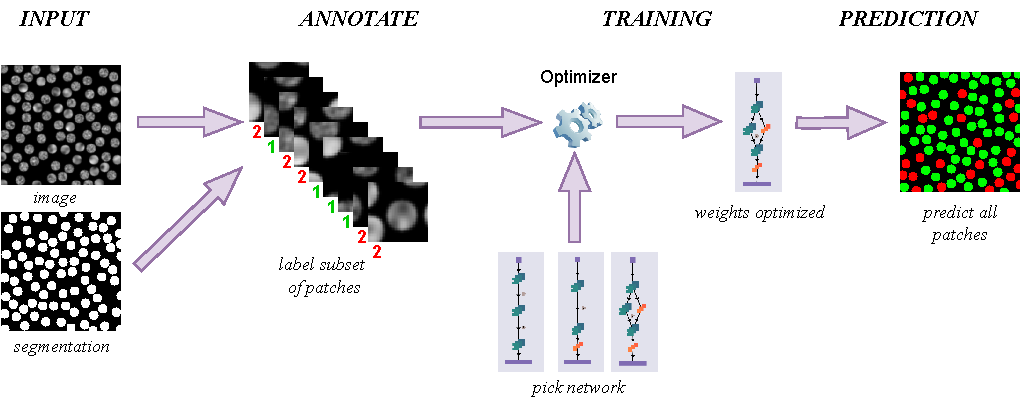
\includegraphics[width=\linewidth]{Figures/pipeline_svetlana.pdf}
  \caption{The SVETLANA plugin pipeline. \label{fig:pipeline}}
\end{figure*}

\subsubsection{The annotation mode}

\begin{wrapfigure}{r}{0.5\linewidth}
 \centering
<<<<<<< HEAD
 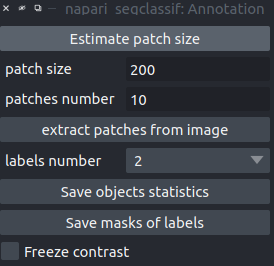
\includegraphics[scale=0.18]{Figures/annotation.png}
  \caption{Annotation interface}
  \label{labelization}
=======
 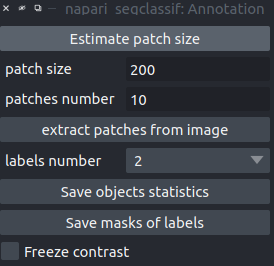
\includegraphics[width=1\linewidth]{Figures/annotation.png}
  \caption{Annotation module. \label{fig:patch}}
\end{wrapfigure}
>>>>>>> 277590bf311dca73b99f19da2214aa7761450383



This first sub-plugin in Fig. \ref{fig:patch} takes as input two images: the image itself and its segmentation mask. The user can also choose the number of different labels he wants.

The connected components of the segmentation mask are then extracted using scikit-image \cite{van2014scikit}. 

Then, there are two possibilities to annotate: 
\begin{itemize}
  \item The user clicks on the desired connected component and labels it. 
  \item SVETLANA randomly picks a connected component, displays it with its neighborhood and the user labels it. This mode can help avoiding a user bias in the choice of the connected components.
\end{itemize}

Once the user feels enough annotations have been proposed, he can save the results in a binary file including the image path, the labels image path, the list of coordinates for each connected component and the associated labels.
Additionally, it is possible to save a new mask per existing label, as well as a binary file that can be reloaded using the torch.load() function. It contains morphological features of interest of each of the objects that were extracted from the connected component analysis.


\subsubsection{The training mode}


Parler de Deep Image Prior (i.e. on peut entraîner avec peu de labels, rasoir d'Ockham, Yann Ollivier).

\paragraph*{The light-weight approach}


For the classification part, we used relatively classical convolutional neural networks such as ResNet18. Nonetheless, the paradigm goes against the classical approach of training neural networks using very large databases.Indeed, we were inspired by the approach put forward in the article Deep Image Prior\cite{lempitsky2018deep} in which they fit a generator network to a single degraded image. They assimilate the reconstruction to a conditional image generation problem and demonstrate that all the information requisite to resolve it is contained in the single degraded input image and in the network chosen for reconstruction.

In section \ref{sec:experiments}, we will show that it is possible to train an efficient classifier model with a few hundred images.

\paragraph*{The features}

In this section, we are going to detail the different features of the training interface shown in figure \ref{training}. The example image shown in the latter is 3D, composed of two channels, and it has been segmented using Cellpose\cite{stringer2021cellpose}.
\begin{figure}[htp!]{}
 \centering
 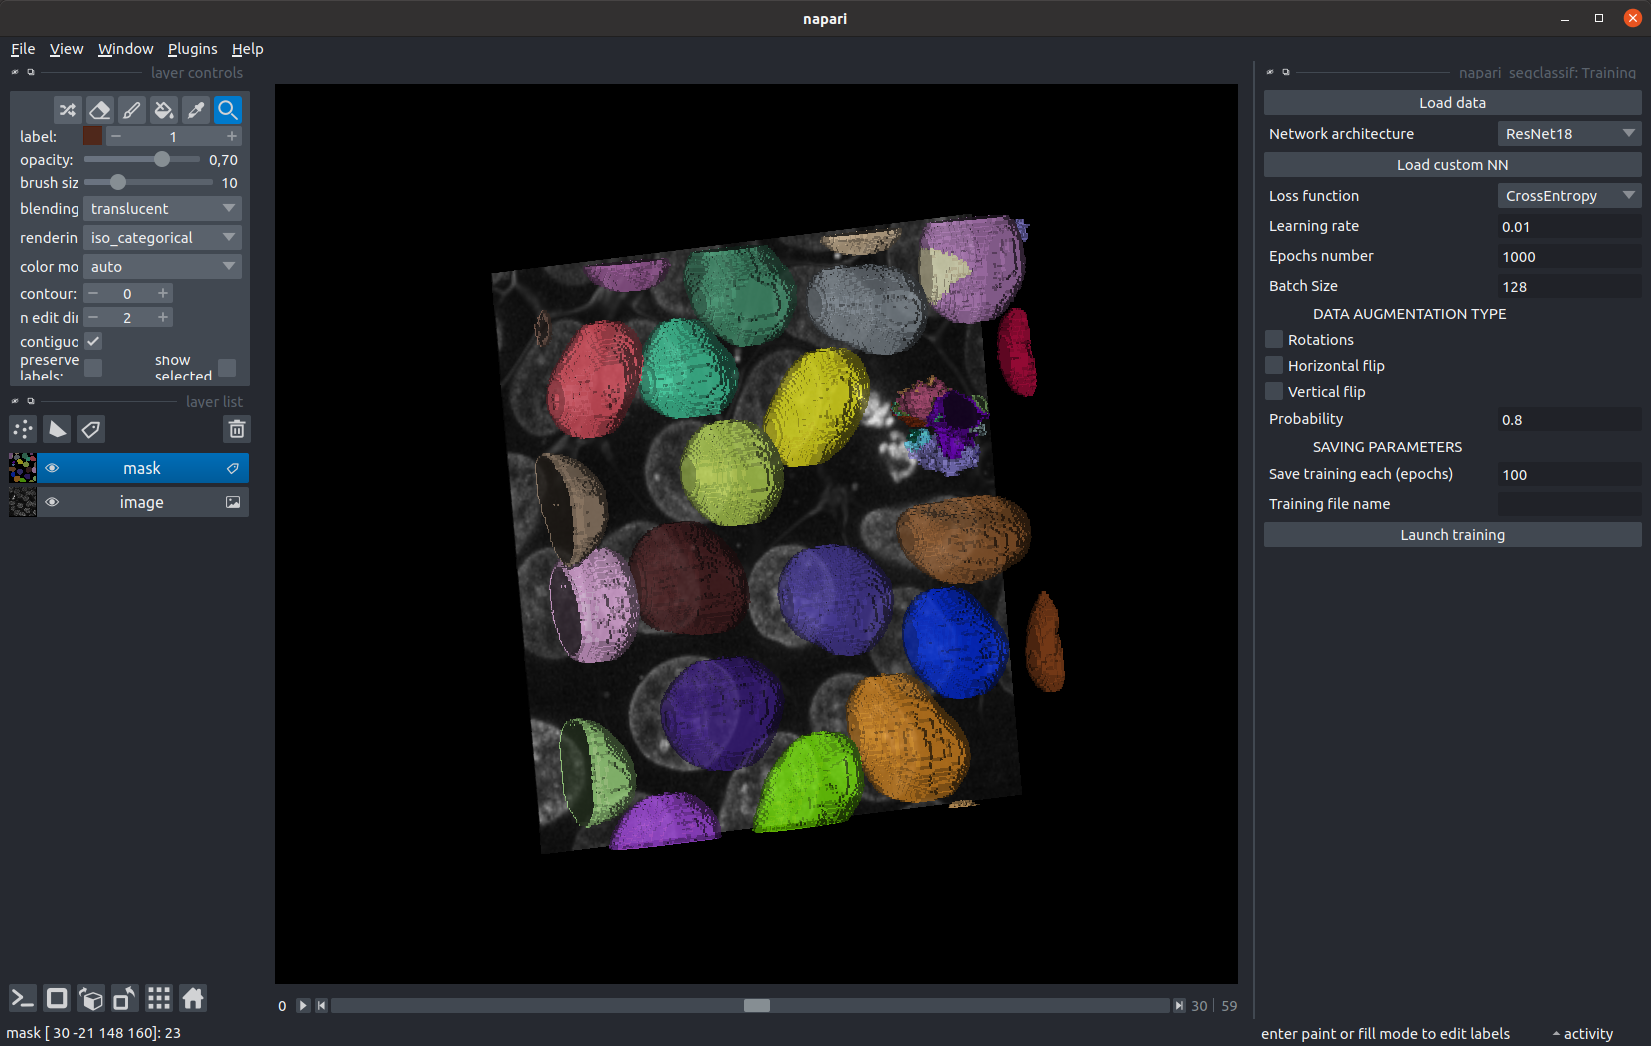
\includegraphics[scale=0.15]{Figures/training.png}
  \caption{The training sub plugin}
  \label{training}
\end{figure}


First of all, the "load data" button aims at loading the content of the binary file saved at the end of the annotation and whose content we have detailed above.

Then, we propose a wide range of network architectures, but the user can also load the custom neural network of one's choice. We suggest the use of the cross entropy loss, but other classical losses are available. 

The learning rate is chosen at the beginning and there is no scheduler for now, which means it will remain constant the whole training. 

As the possible batch size depends on the performance of the machine the user works on, it can be chosen by the user. If it is selected too large, it will be automatically adjusted to the highest power of 2 tolerated by the GPU ram.

Basic data augmentations such as vertical and horizontal flips and rotations of angle between -90° and 90° are available, and their probability of occurrence can be adjusted. 

Finally, we can choose the name of the ".pth" file containing the training result and all the times we want to save. This gives the possibility to access the network at different stages since we have no preconceived notion of the number of epochs necessary for convergence.

The saved files is also a binary containing several data including: the model, the optimizer state, the loss, the epochs number, the loss value, the image path, the labels image path, the patch size.

\subsubsection{The prediction mode}

This plugin is very minimalist, as shown in figure \ref{predict}. Indeed, it allows to load the training result file and to launch the prediction by choosing the batch size. As for the training, the optimal batch size will depend on the capabilities of the GPU.

\begin{figure}[htp!]{}
 \centering
 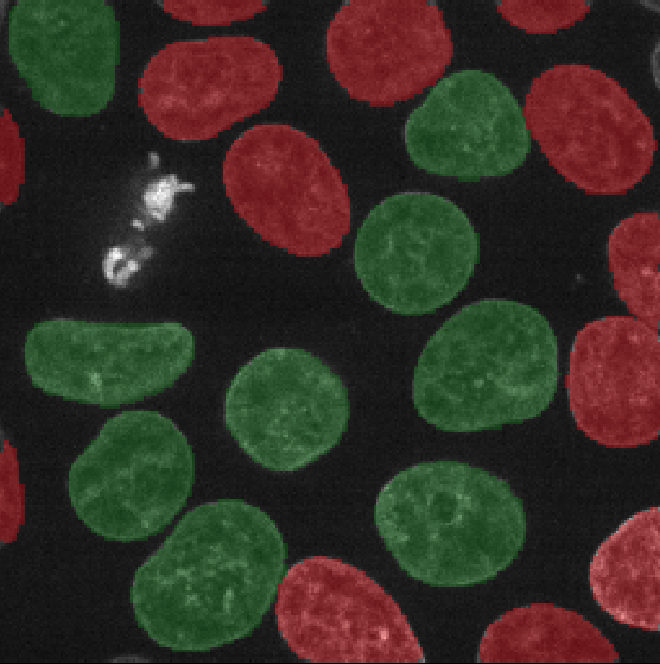
\includegraphics[scale=0.15]{Figures/resultat.png}
  \caption{Example of a 2D prediction with two labels}
  \label{predict}

\end{figure}


\begin{figure}[h!]{}
 \centering
 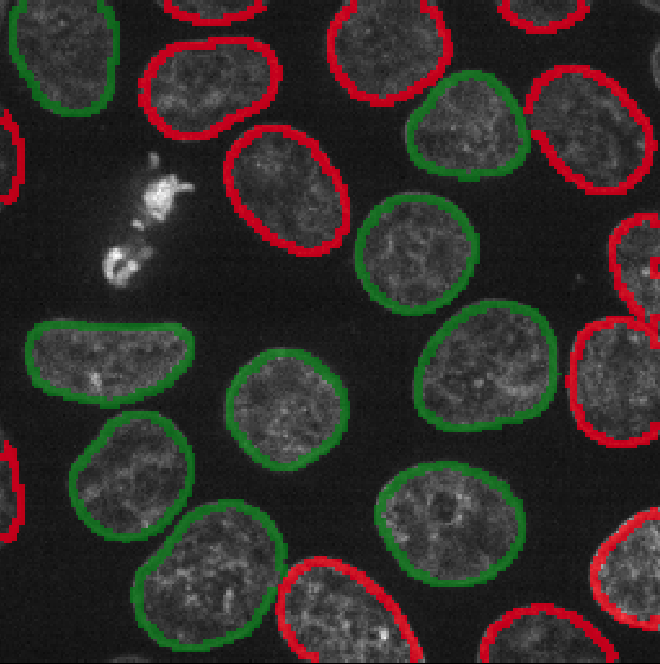
\includegraphics[scale=0.15]{Figures/resultat_contour.png}
  \caption{An alternative representation of the labels}
  \label{predict_contours}

\end{figure}

In 2D, there are two representations of the classified mask as shown in figures \ref{predict} and \ref{predict_contours}.

As for the annotation plugin, the user has the opportunity to save a mask per label and a binary file containing relevant morphological information about the classified objects to perform further statistical analysis.


\section{Numerical Experiments}
\label{sec:experiments}


\subsection{First experiment: artificial texture classification}

For this first experiment, we generated an image composed of  345 circular objects differentiable only by their texture that we seek to order into two classes. The distribution of the two textures in the image is about 70/30 and we extract 100 thumbnails to annotate. 
As we have very few data, we decided to demonstrate the efficiency of shallow convolutional networks. As shown in Figure \ref{CNN2D}, we designed a 2-layer CNN of 3000 parameters only.

Training 500 epochs, i.e. a calculation time of 20 seconds, with a constant learning rate of 0.01, we get a misclassified objects rate of 0.8\%.


\begin{figure}[h!]{}
 \centering
 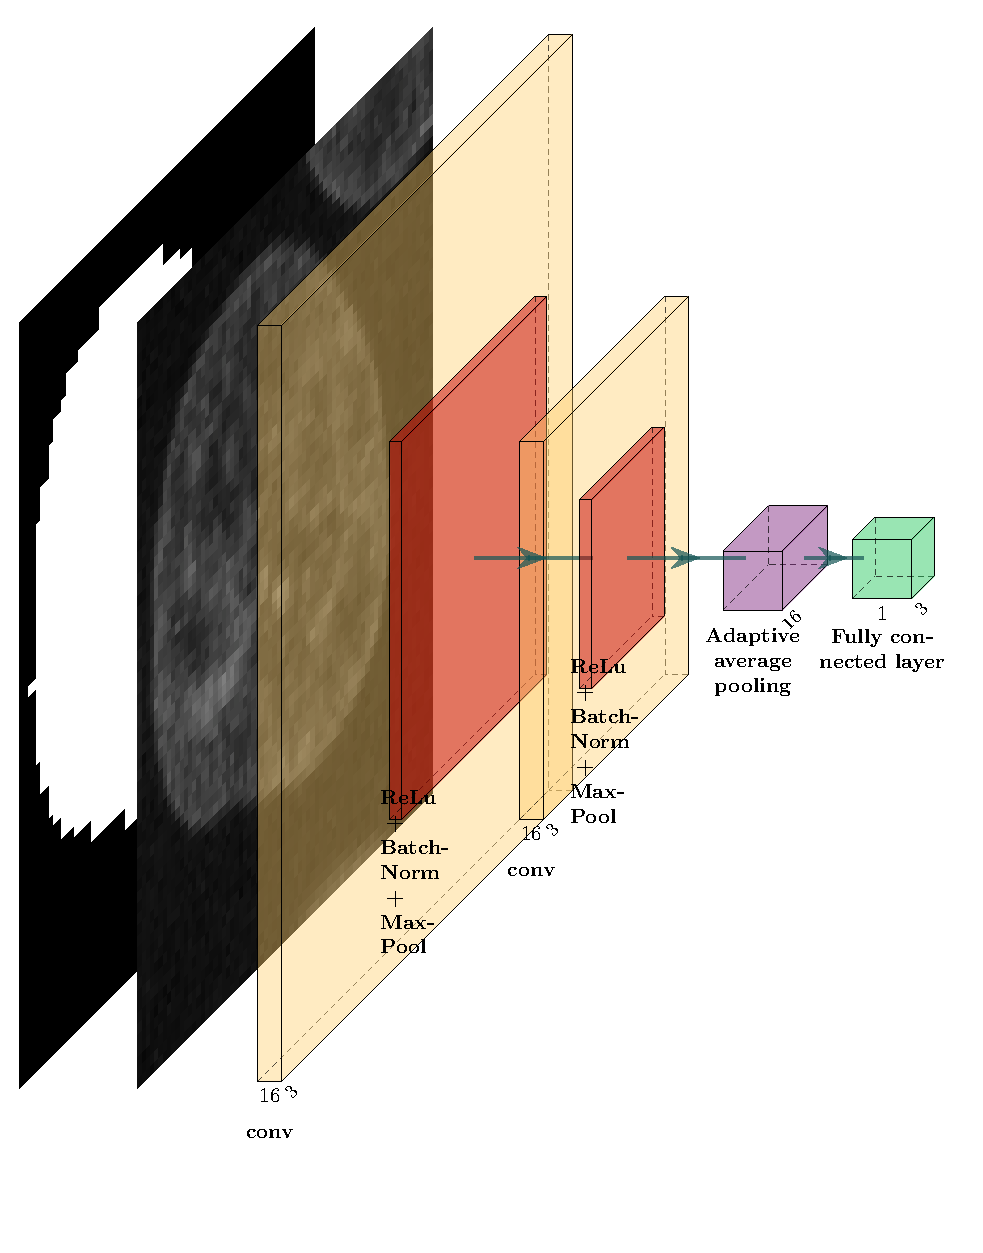
\includegraphics[scale=0.35]{Figures/myfirstcnn.pdf}
  \caption{Our 2-layer custom CNN}
  \label{CNN2D}

\end{figure}


\begin{figure}[h!]
  \begin{center}
    \subfloat[Original texture image]{
      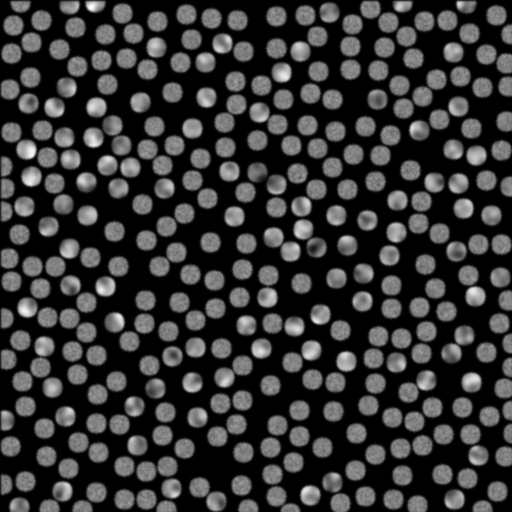
\includegraphics[scale=0.25875]{Figures/textures.png}
      \label{textures}
                         }
    \subfloat[Classified mask]{
      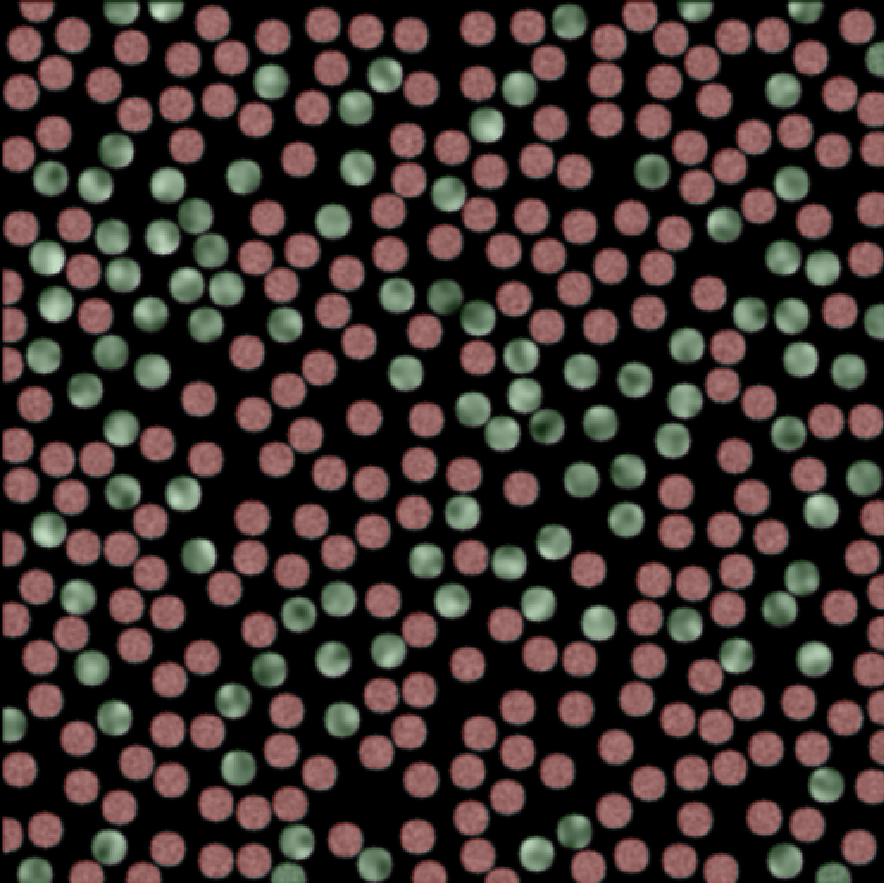
\includegraphics[scale=0.15]{Figures/textures_res.png}
      \label{textures res}
                         }
     \end{center}
\caption{Result of the textures classification}
\end{figure}


\subsection{Second experiment: Infected cells detection in virology}

This image depicts cells that are, for some, infected with an adenovirus. It is composed of:
\begin{itemize}
  \item a first channel containing a Hoechst labeling of the nuclei
  \item a second channel where the sites of viral proliferation have been marked using the ANCHOR system and which will serve as our ground truth.
\end{itemize}
We annotated 100 cells over 245 to train our 2-layer model and got a rate of 95.5\% of well-classified cells.    


\begin{figure}[h!]
  \begin{center}
    \subfloat[Hoechst staining]{
      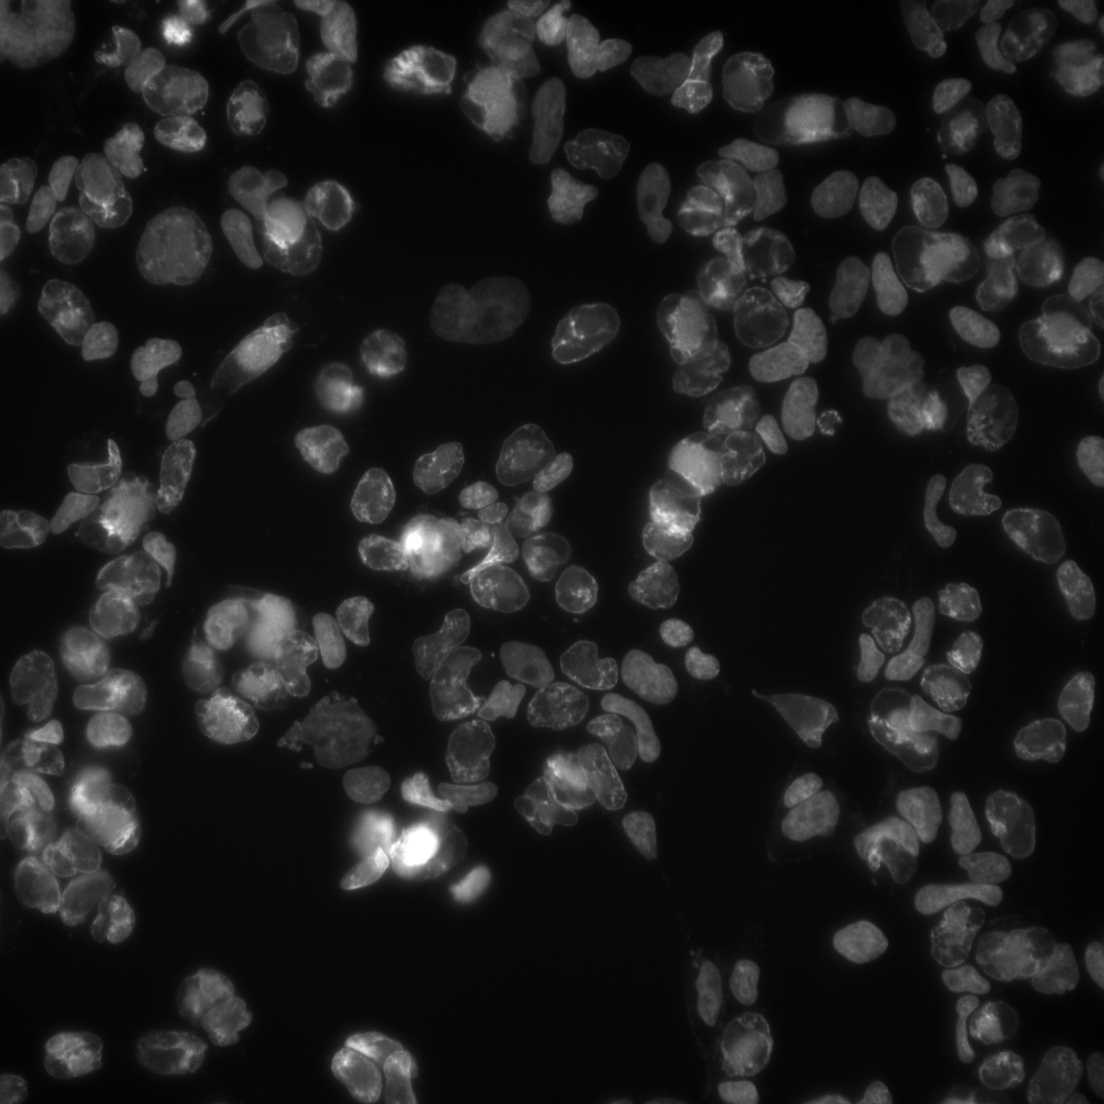
\includegraphics[scale=0.07]{Figures/viro_canal0.png}
      \label{textures}
                         }
    \subfloat[ANCHOR channel]{
      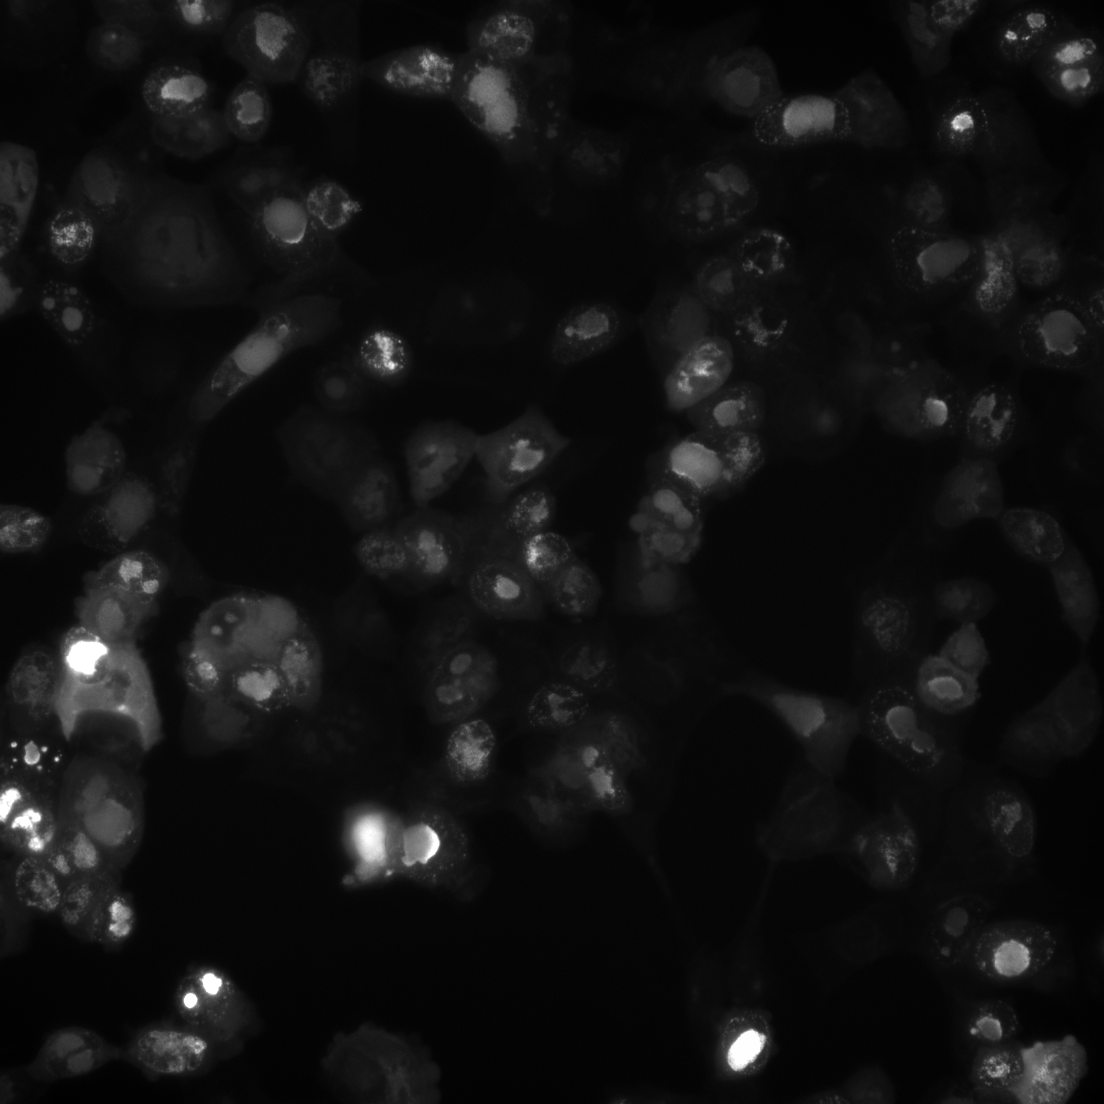
\includegraphics[scale=0.07]{Figures/viro_canal1.png}
      \label{textures res}
                         }
   \subfloat[classification result]{
      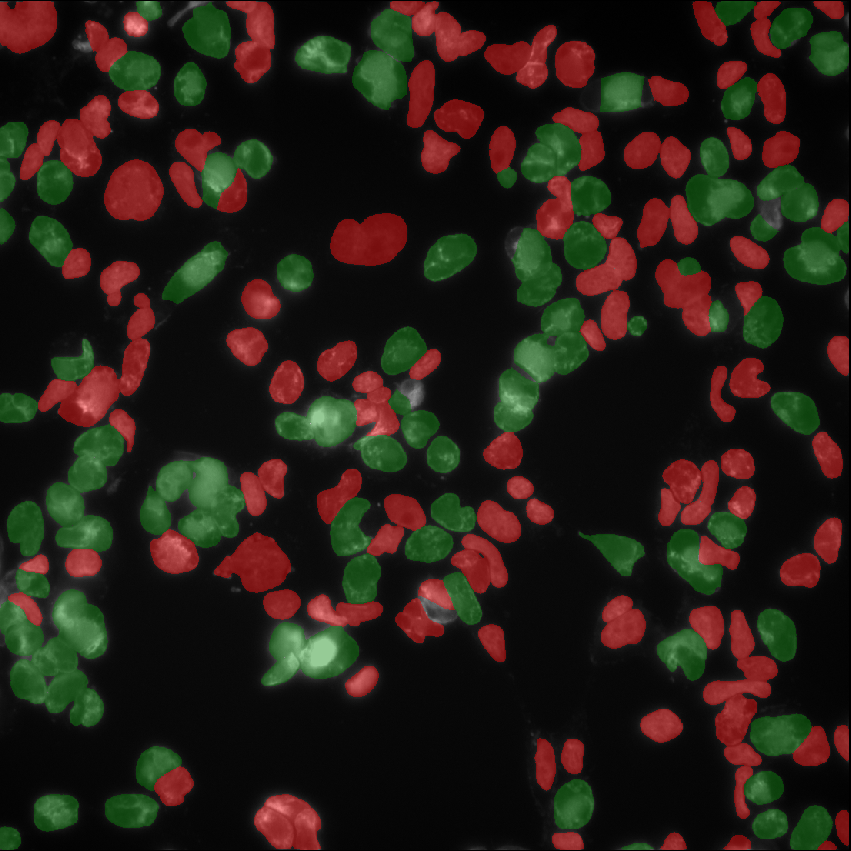
\includegraphics[scale=0.091]{Figures/resultat_viro.png}
      \label{textures res}
                         }
     \end{center}
\caption{Result of the infected cells classification}
\end{figure}


\subsection{Third experiment: ABS}


\begin{figure}[h!]
  \begin{center}
    \subfloat[ABS image]{
      \includegraphics[scale=0.0445]{Figures/Image_ABS.png}
      \label{ABS image}
                         }
    \subfloat[Zoomed crop in the image showing the cells variety]{
      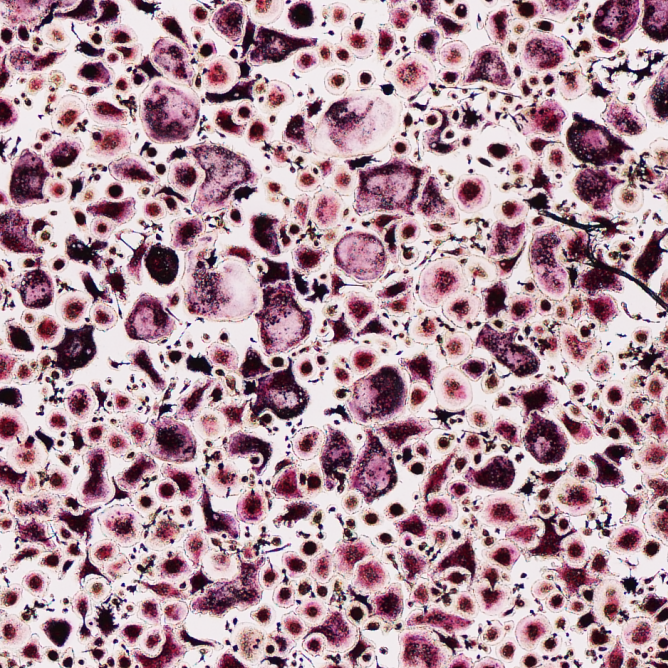
\includegraphics[scale=0.16]{Figures/crop_ABS.png}
      \label{Zoomed crop}
                         }
     \end{center}
\caption{ABS image to segment and classify}
\end{figure}



\begin{figure}[h!]
  \begin{center}
    \subfloat[Good cell]{
      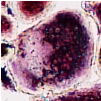
\includegraphics[scale=0.4]{Figures/good1.png}
      \label{Good cell1}
                         }
    \subfloat[Good cell]{
      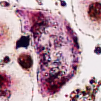
\includegraphics[scale=0.4]{Figures/good2.png}
      \label{Good cell2}
                         }
   \subfloat[Bad cell]{
      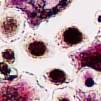
\includegraphics[scale=0.4]{Figures/bad1.png}
      \label{Bad cell1}
                         }
    \subfloat[Bad cell]{
      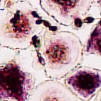
\includegraphics[scale=0.4]{Figures/bad2.png}
      \label{Bad cell2}
                         }
     \end{center}
\caption{ABS image to segment and classify}
\end{figure}



\begin{figure}[h!]{}
 \centering
 \includegraphics[scale=0.0445]{Figures/res_ABS.png}
  \caption{Resultat classification}
  \label{res ABS}

\end{figure}

4591 kept over 16671 after classification.


\section{Conclusion}
\label{sec:conclusion}

We showcased through various applications that SVETLANA is already a handful tool for analyzing segmentation results. 
It is yet at an early stage of development. By publishing this paper, we wished to have a first document that could be cited in the case that the plugin was used successfully. We plan to progressively add new features suggested by users or our own experience, to make this tools as helpful as possible to the community. 
\begin{itemize}
  \item Add the ability to label multiple images. 
  \item Add the ability to directly label or correcting the labels by clicking on the connected components. 
  \item Add the ability to predict on multiple images. 
%  \item Add new neural network architectures. 
  \item Add a layer with already annotated features.
\end{itemize}

% To start a new column (but not a new page) and help balance the last-page
% column length use \vfill\pagebreak.
% -------------------------------------------------------------------------
\vfill
\pagebreak

% \section{REFERENCES}
% \label{sec:ref}

% References should be produced using the bibtex program from suitable
% BiBTeX files (here: refs). The IEEEbib.bst bibliography
% style file from IEEE produces unsorted bibliography list.
% -------------------------------------------------------------------------
\bibliographystyle{IEEEbib}
\bibliography{refs}

\end{document}
























%%%%%%%%%%%%%%%%%%%%%%%%%%%%%%%%%%%%%%%%%%%%%%%%%%%%%%%%%%%%%%%%%%%%

La dernière décennie a rendu la segmentation automatique d'images bio-médicales bien plus accessible à des utilisateurs non experts en traitement du signal. 
Ceci est largement dû aux progrès en apprentissage automatique et notamment en apprentissage par réseaux de neurones convolutionnels. Ils permettent notamment d'éviter le réglage de nombreux hyperparamètres dont le tuning est difficile et dont la signification est obscure pour les non initiés. 
A titre d'exemple, on peut citer des outils récents, puissants et populaires tels que Ilastik \cite{berg2019ilastik}, Cellpose \cite{stringer2021cellpose}, StarDist \cite{fazeli2020automated} ou plus récemment Deep-ImageJ \cite{gomez2021deepimagej}. 

Malheureusement, les résultats de segmentation -- aussi bons soient-t'ils -- sont rarement exploitables directement pour répondre à des questions biologiques. Il est en effet fréquent qu'il faille  classifier les objets détectés pour effectuer des analyses statistiques apportant un sens concret aux résultats. En un sens, ces outils ont résolu une partie du problème, mais une partie importante et difficile de l'analyse reste inaccessible.

L'objectif de ce travail est de continuer à combler le fossé entre les progrès méthodologiques et les end-users, en fournissant des outils faciles d'utilisation pour la classification des résultats de segmentation.
Ces outils prennent la forme d'un plugin Napari \cite{perkel2021python}, qui est un nouvel outil de visualisation d'images complexes sous Python.

